\chapter{Конструкторский раздел}
\label{cha:design}

В данном разделе будут приведены схемы алгоритма полного перебора и муравьиного алгоритма для решения задачи коммивояжера, приведено описание используемых типов данных, классов эквивалентности, а также описана структура ПО.

\section{Схемы алгоритмов}

На рис. \ref{fig:ant_alg_scheme} - \ref{fig:full_comb_alg_scheme} приведены схемы алгоритмов для решения задачи коммивояжера (полного перебора и муравьиного алгоритма).

\begin{figure}[h]
	\centering
	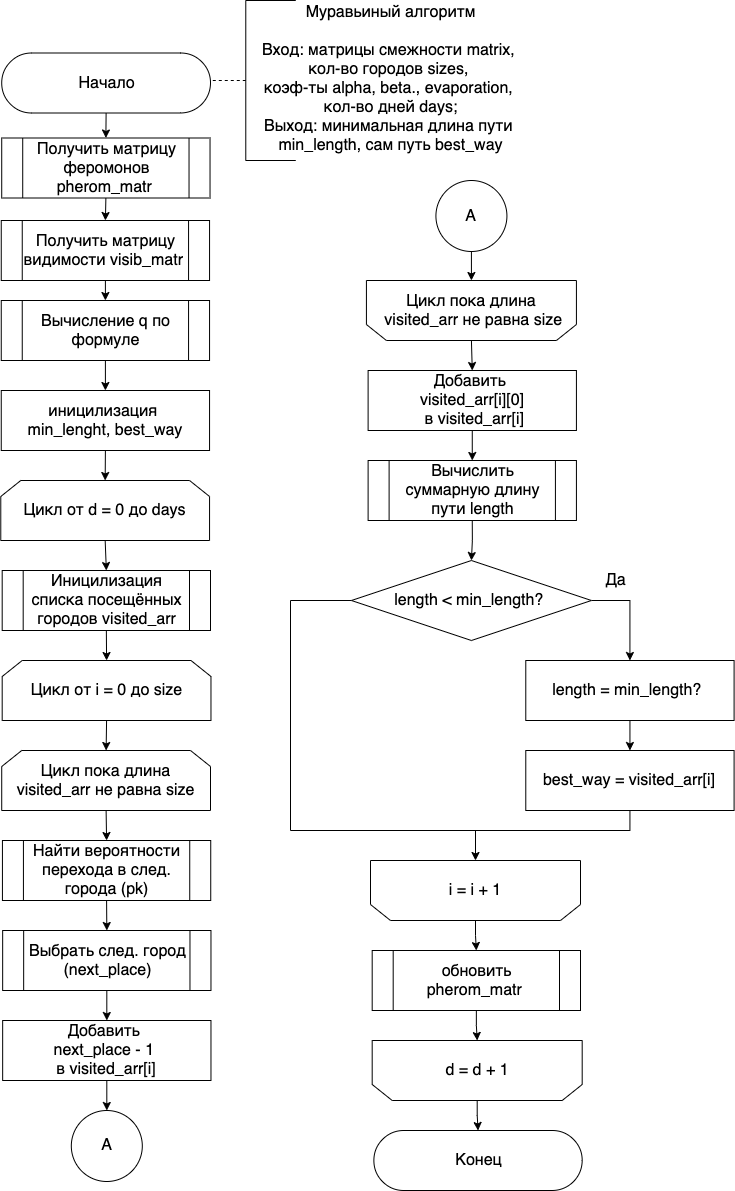
\includegraphics[scale=0.55]{img/ant_alg_scheme.png}
	\caption{Схема муравьиного алгоритма}
	\label{fig:ant_alg_scheme}
\end{figure}

\clearpage

\begin{figure}[h]
	\centering
	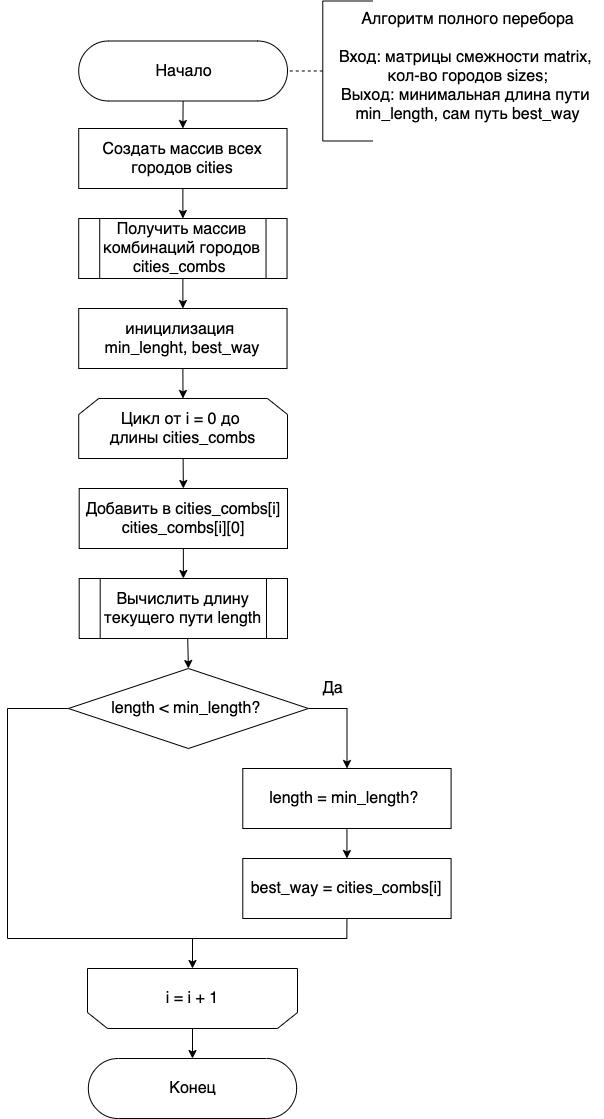
\includegraphics[scale=0.6]{img/full_comb_alg_scheme.png}
	\caption{Схема алгоритма полного перебора}
	\label{fig:full_comb_alg_scheme}
\end{figure}

\clearpage

\section{Классы эквивалентности}

Выделенные классы эквивалентности для тестирования:

\begin{itemize}
	\item коэффицент $\alpha$ <= 0;
	\item коэффицент $\alpha$ не является числом;
	\item коэффицент $\beta$ <= 0;
	\item коэффицент $\beta$ не является числом;
	\item коэффицент $evaporation$ <= 0;
	\item коэффицент $evaporation$ не является числом;
	\item номер команды < 0 или > 5;
	\item номер команды не является целым числом;
	\item корректный ввод всех параметров;
\end{itemize}

\section{Описание используемых типов данных}

При реализации алгоритмов будут использованы следующие структуры данных:

\begin{itemize}
	\item размер матрицы смежности - целое число типа $int$;
	\item матрица смежности - матрица, элементы которой имеют тип $int$;
	\item коэффиценты $\alpha$, $\beta$, $evaporation$ - действительные числа типа $float$;
	\item название файла - строка типа $str$.
\end{itemize}

\section{Структура ПО}

ПО будет состоять из следующих модулей:

\begin{itemize}
	\item $main.py$ -- файл, содержащий функцию $main$;
	\item $generate.py$ -- файл, содержащий функцию для генирации матриц;
    \item $ant\_algorythm.py$ -- файл, в котором содержатся функции муравьиного алгоритма для решения задачи коммивояжера;
    \item $full\_combinations.py$ -- файл, в котором содержатся функции алгоритма полного перебора для решения задачи коммивояжера;
    \item $parametrization.py$ -- файл, содержащий функцию параметризации для муравьиного алгоритма;
    \item $compare\_time.py$ -- файл, в котором содержатся функции для замера времени работы алгоритмов и построения графика зависимоти времени выполнения от размера матрицы;
    \item $read\_print.py$ -- файл, в котором содержатся функции ввода вывода данных;
    \item $color.py$ -- файл, который содержит переменные типа $string$ для цветного вывода результата работы программы в консоль.
\end{itemize}

\section{Вывод}

В данном разделе на основе теоретических данных были построены схемы требуемых алгоритмов решения задачи коммивояжера (муравьиного алгоритма и алгоритма полного перебора), выбраны используемые типы данных, выделены классы эквивалентности для тестирования, а также была описана структура ПО.

%%% Local Variables:
%%% mode: latex
%%% TeX-master: "rpz"
%%% End:
